% ---------------------------------------------------------------------------- %
\begin{figure}
  \centering
	\subfigure[\label{fig:conclusions:end:3}]
	{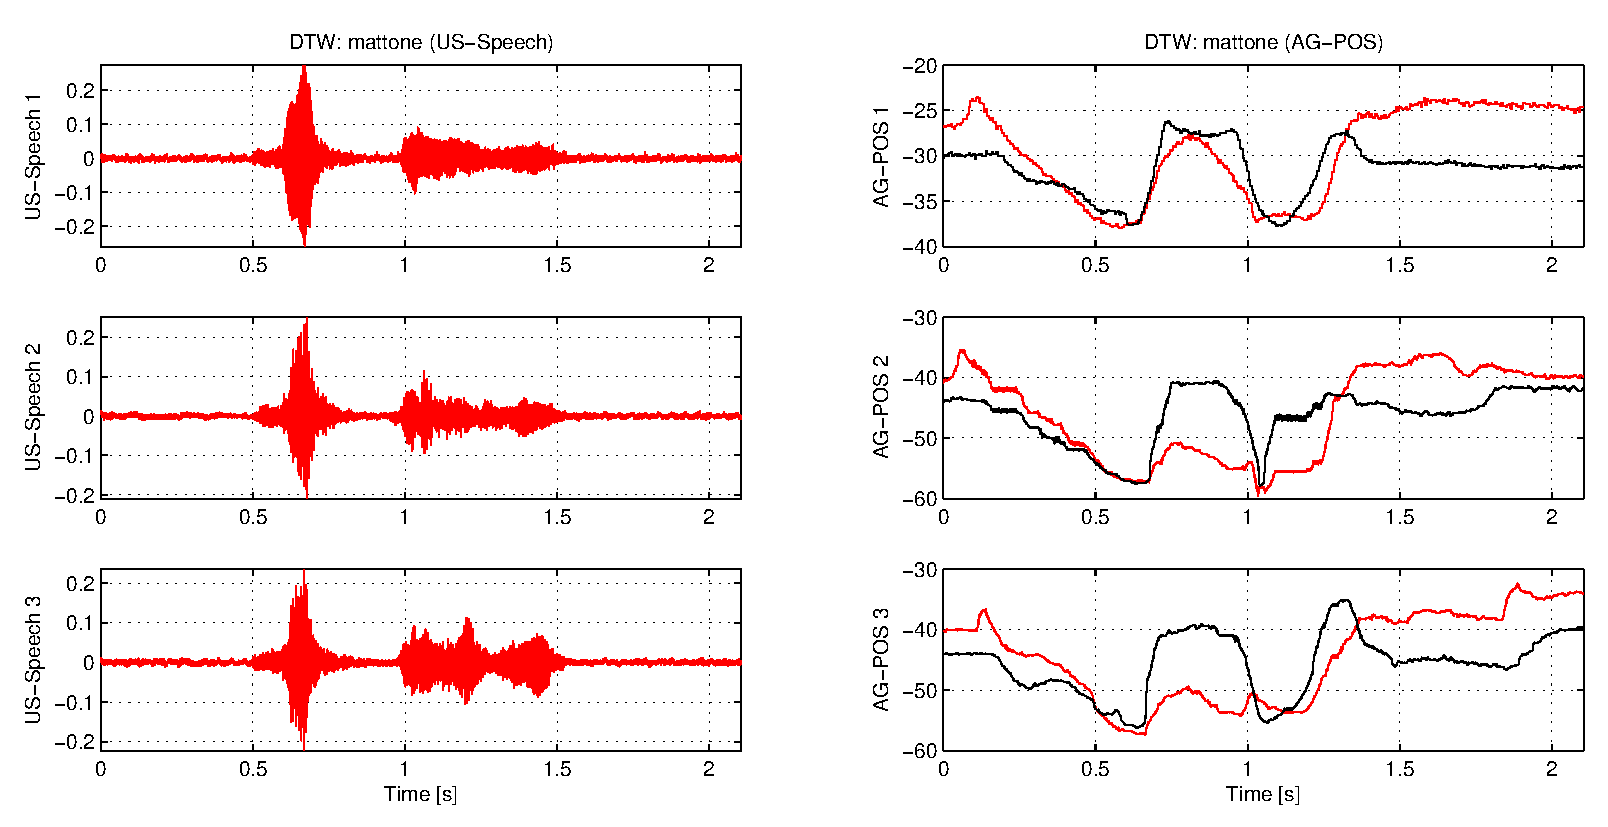
\includegraphics[width=\textwidth]{include/conclusions/images/end_same_dtw.eps}}
	
	\subfigure[\label{fig:conclusions:end:4}]
	{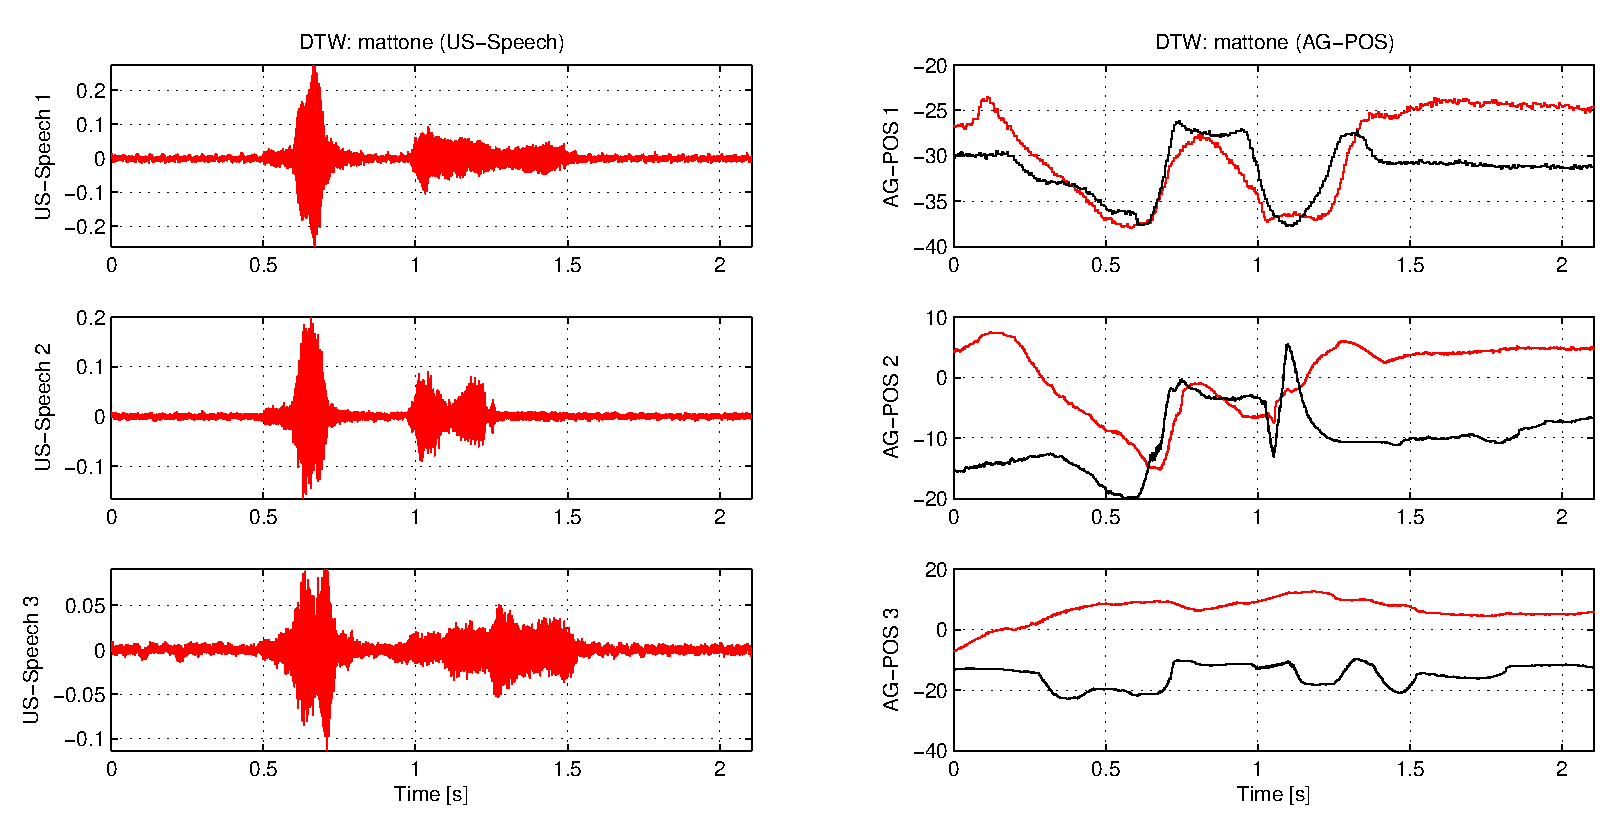
\includegraphics[width=\textwidth]{include/conclusions/images/end_diff_dtw.eps}}

	\caption[Speech signals and tongue vertical displacement (Dynamic Time Warp)]
	{\textbf{Speech signals and tongue vertical displacement (Dynamic Time Warp)}:
	this Figure is analogous to Figure~\ref{fig:conclusions:end}. The only
	difference consist in warping the signals by the means of the DTW algorithm.}
	\label{fig:conclusions:end:dtw}
\end{figure}
% ---------------------------------------------------------------------------- %
